% Plantilla SIPAGRE — 1° PARTE (1S) PERSONALIZADA
% =================================================
% Generada a partir del template original con los siguientes cambios:
%   - Se añade \usepackage{graphicx} para incluir el QR
%   - Se acorta la línea "DOCUMENTO IDENTIDAD" (3 cm en vez de 6 cm)
%   - Se añade un QR de 20mm × 20mm en el extremo derecho del título box
%   - Se imprimen automáticamente Nombre, ID, Curso del estudiante
%
% Placeholders (rellenados por Python antes de compilar):
%   <<NOMBRE>>   Nombres y apellidos del estudiante (mayúsculas)
%   <<ID>>       Documento de identidad
%   <<CURSO>>    Curso (ej. 1101)
%   <<SESION>>   "1S"
%   <<QR_PATH>>  Ruta absoluta del PNG del QR
%
% NO se modifica nada de las columnas de respuestas ni de los timing marks,
% para que el OMR existente siga funcionando sin recalibrar.

\documentclass[letterpaper]{article}
\usepackage[top=1.1cm, bottom=0.9cm, left=1.2cm, right=1.1cm]{geometry}
\usepackage{tikz}
\usepackage{graphicx}                                            % <-- NUEVO (para el QR)
\usetikzlibrary{calc, shapes.geometric, positioning}
\usepackage[T1]{fontenc}
\usepackage[utf8]{inputenc}
\usepackage{helvet}
\renewcommand{\familydefault}{\sfdefault}
\setlength{\parindent}{0pt}
\setlength{\parskip}{0pt}
\pagestyle{empty}

%================= AJUSTE FINO OMR =================
\newlength{\TMw}    \setlength{\TMw}{6pt}
\newlength{\Nw}     \setlength{\Nw}{14pt}
\newlength{\Bdia}   \setlength{\Bdia}{12pt}
\newlength{\Bsep}   \setlength{\Bsep}{1.5pt}
\newlength{\Brad}   \setlength{\Brad}{6pt}
\newlength{\Rowsep} \setlength{\Rowsep}{2pt}

% ================= ESTILO CUADROS REDONDEADOS =================
\tikzset{cuadrocolumna/.style={
    draw,
    draw=black!70,
    line width=1.2pt,
    rounded corners=10pt,
    inner sep=8pt,
    outer sep=0pt,
    fill=white,
    align=left,
    anchor=north,
    text width=\linewidth-16pt
}}

%================= BURBUJA =================
\newcommand{\B}{%
  \makebox[\Bdia][c]{%
    \tikz[baseline=-2.8pt]{%
      \filldraw[fill=white, draw=black!70, line width=0.7pt, rounded corners=0pt, solid]
        (0,0) circle (\Brad);}%
  }%
}

%================= TIMING MARK =================
\newcommand{\TM}{%
  \makebox[\TMw][c]{%
    \tikz[baseline=-4pt]{\fill[black, rounded corners=0pt, solid](0,-5pt) rectangle (\TMw,5pt);}%
  }%
}

%================= FILAS =================
\newcommand{\Q}[1]{%
  \noindent
  \TM\hspace{1pt}%
  \makebox[\Nw][r]{\scriptsize\textbf{#1.}}%
  \hspace{2pt}%
  \B\hspace{\Bsep}\B\hspace{\Bsep}\B\hspace{\Bsep}\B%
  \par\vspace{\Rowsep}%
}

\newcommand{\QH}[1]{%
  \noindent
  \TM\hspace{1pt}%
  \makebox[\Nw][r]{\scriptsize\textbf{#1.}}%
  \hspace{2pt}%
  \B\hspace{\Bsep}\B\hspace{\Bsep}\B\hspace{\Bsep}\B\hspace{\Bsep}%
  \B\hspace{\Bsep}\B\hspace{\Bsep}\B\hspace{\Bsep}\B%
  \par\vspace{\Rowsep}%
}

%================= HEADERS COLUMNAS =================
\newcommand{\HDR}{%
  \noindent
  \hspace{\TMw}\hspace{1pt}\hspace{\Nw}\hspace{2pt}%
  \foreach \L in {A,B,C,D}{%
    \makebox[\Bdia][c]{\footnotesize\textbf{\L}}\hspace{\Bsep}%
  }%
  \par\vspace{2pt}%
}

\newcommand{\HDRH}{%
  \noindent
  \hspace{\TMw}\hspace{1pt}\hspace{\Nw}\hspace{2pt}%
  \foreach \L in {A,B,C,D,E,F,G,H}{%
    \makebox[\Bdia][c]{\footnotesize\textbf{\L}}\hspace{\Bsep}%
  }%
  \par\vspace{2pt}%
}

\begin{document}

%================= MARCADORES DE PÁGINA =================
\begin{tikzpicture}[remember picture, overlay]
  \fill[black] ($(current page.north west)+(8mm,-8mm)$)  rectangle ++(8mm,-8mm);
  \fill[black] ($(current page.north east)+(-8mm,-8mm)$) rectangle ++(-8mm,-8mm);
  \fill[black] ($(current page.south west)+(8mm,16mm)$)  rectangle ++(8mm,8mm);
  \fill[black] ($(current page.south east)+(-8mm,16mm)$) rectangle ++(-8mm,8mm);
\end{tikzpicture}

\vspace*{2mm}

% ================== ENCABEZADO PRINCIPAL (MODIFICADO) ==================
\noindent\makebox[\textwidth][c]{
\begin{tikzpicture}[x=1cm, y=1cm]

% --- Caja principal (5mm más alta que el original para acomodar el QR) ---
\draw[line width=2pt, rounded corners=10pt] (-9, -2.1) rectangle (9, -5.0);

% --- Título (font reducido a \large para no colisionar con el QR) ---
\node[font=\large\bfseries, align=center] at (0, -2.50)
  {SIPAGRE - SIMULACRO PARA GRANDES RETOS 1° PARTE};

% --- IZQUIERDA: Nombre del estudiante ---
% Nombre PRE-IMPRESO encima de la línea
\node[font=\normalsize, anchor=south] at (-4.75, -3.46) {<<NOMBRE>>};
\draw[line width=1.5pt] (-8, -3.5) -- (-1.5, -3.5);
\node[font=\normalsize\bfseries] at (-4.55, -4.0) {NOMBRES Y APELLIDOS};

% --- CENTRO: Logo "Pruebas Saber 11°" (sin cambios) ---
\begin{scope}[shift={(0, -3.5)}]
    \fill[black] (-1.3, 0.7) -- (-0.9, 0.3) -- (-0.5, 0.7) -- (-0.5, 0.45) -- (-0.9, 0.05) -- (-1.3, 0.45) -- cycle;
    \fill[black] (-1.3, 0.3) -- (-0.9, -0.1) -- (-0.5, 0.3) -- (-0.5, 0.05) -- (-0.9, -0.35) -- (-1.3, 0.05) -- cycle;
    \node[anchor=west, align=left, inner sep=0] at (-0.3, 0.2) {\fontsize{6}{7}\selectfont Pruebas\\[-0.5ex]\large\bfseries Saber};
    \fill[black!90] (1.6, 0.2) circle (0.45);
    \node[text=white, font=\bfseries\normalsize] at (1.6, 0.2) {11$^\circ$};
\end{scope}

% --- DOCUMENTO (línea acortada de 6cm → 3cm para liberar espacio al QR) ---
% ID PRE-IMPRESO encima de la línea
\node[font=\normalsize, anchor=south] at (4.0, -3.46) {<<ID>>};
\draw[line width=1.5pt] (2.5, -3.5) -- (5.5, -3.5);
\node[font=\normalsize\bfseries] at (4.0, -4.0) {DOC. IDENTIDAD};

% --- NUEVO: QR + etiqueta CURSO/SESIÓN en el extremo derecho ---
% QR de 20mm × 20mm centrado en (7.5, -3.45)
\node[anchor=center] at (7.5, -3.45) {%
  \includegraphics[width=2.0cm]{<<QR_PATH>>}};
% Etiqueta legible debajo del QR (dentro de la caja)
\node[font=\footnotesize\bfseries, anchor=center] at (7.5, -4.75)
  {CURSO <<CURSO>> · <<SESION>>};

\end{tikzpicture}
}

\vspace{6mm}

%================= RESPUESTAS (IDÉNTICAS AL ORIGINAL) =================
\noindent
% Columna 1
\begin{minipage}[t]{0.20\textwidth}
  \vspace{0pt}
  \noindent
  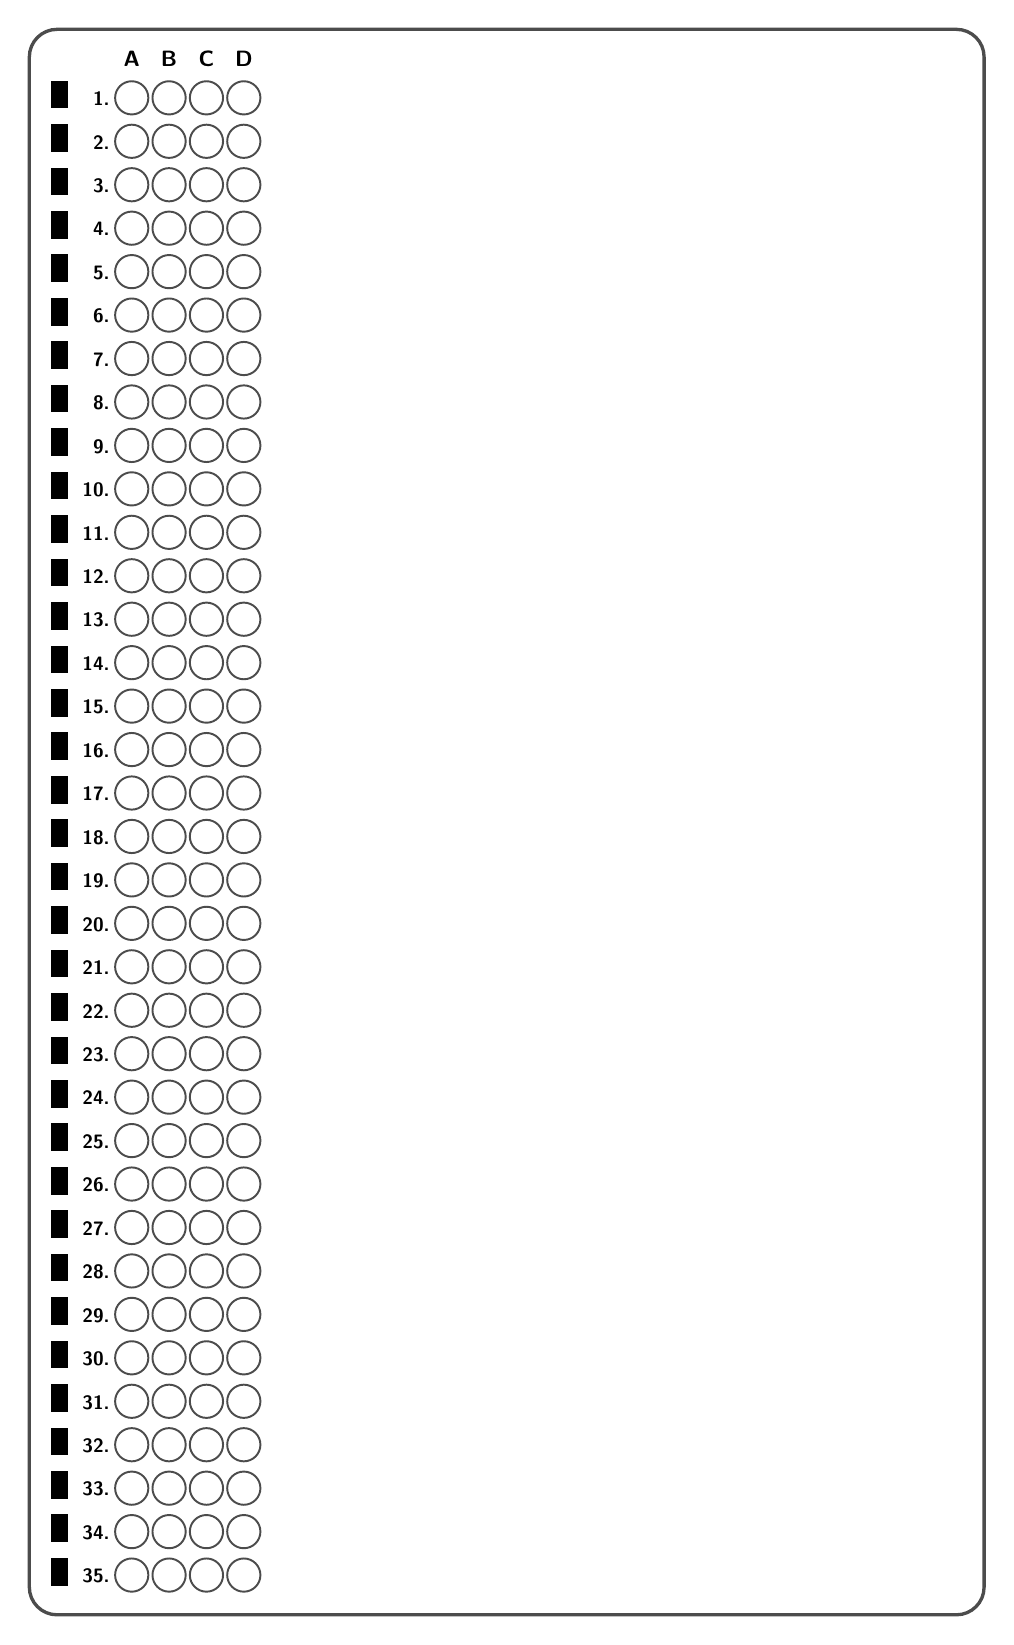
\begin{tikzpicture}
    \node[cuadrocolumna] {
        \HDR
        \foreach \n in {1,...,35}{\Q{\n}}
    };
  \end{tikzpicture}
\end{minipage}%
\hfill
% Columna 2
\begin{minipage}[t]{0.20\textwidth}
  \vspace{0pt}
  \noindent
  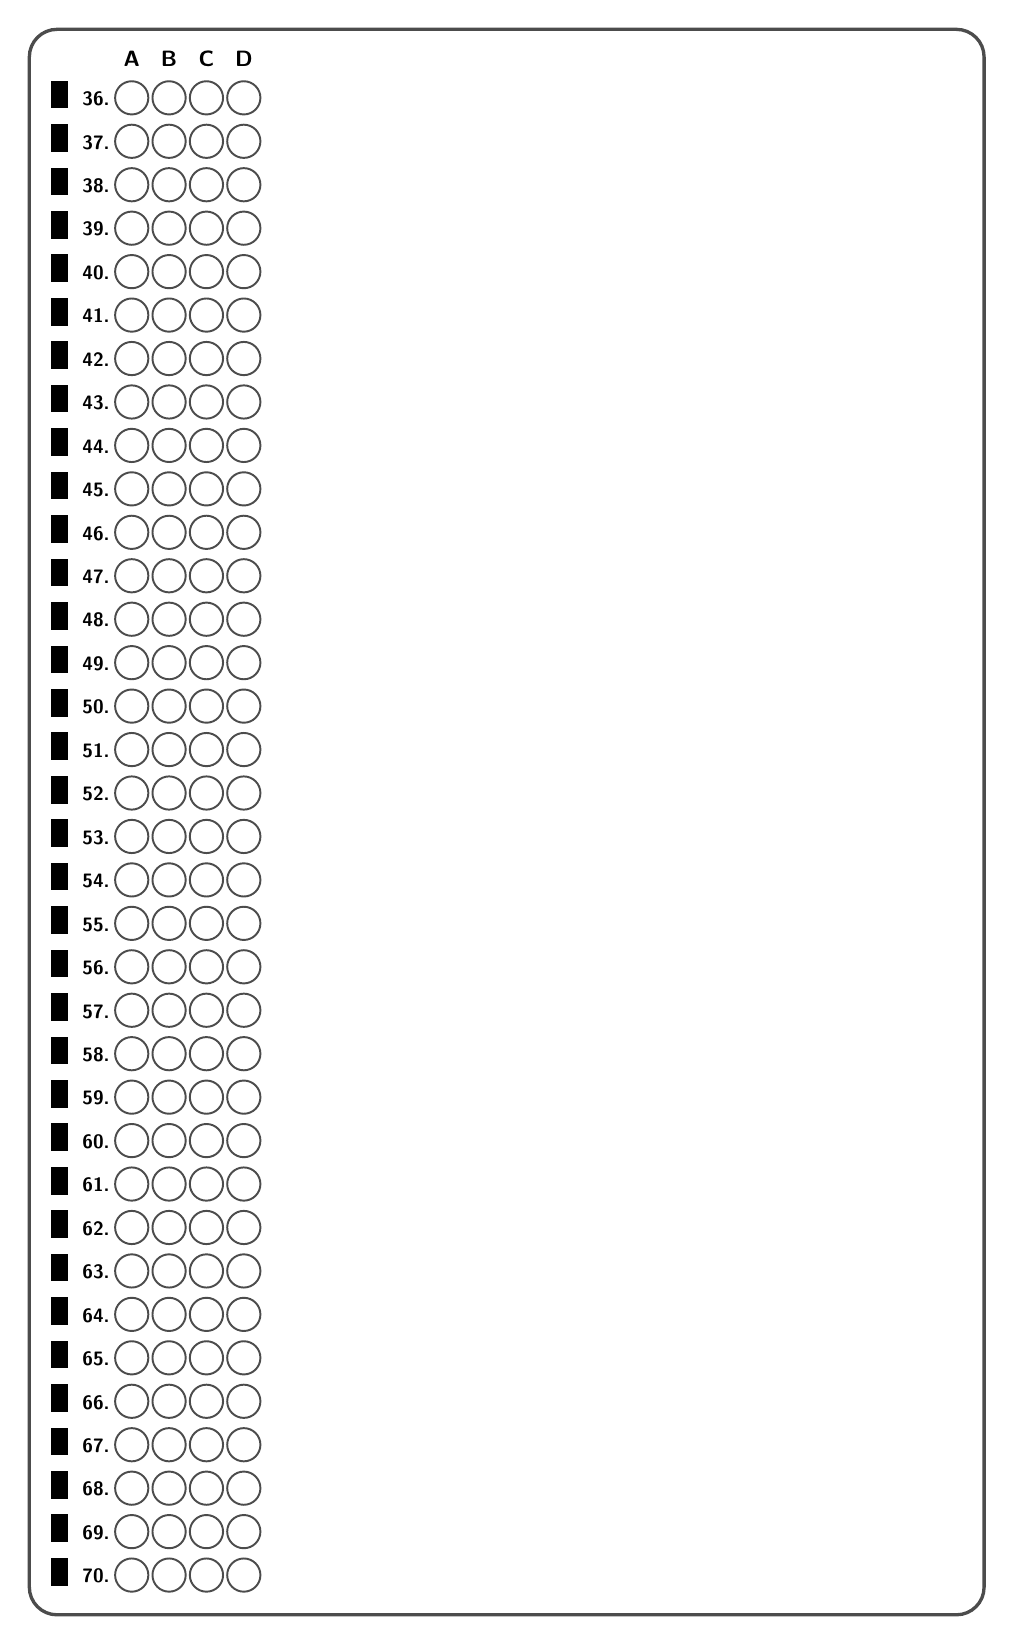
\begin{tikzpicture}
    \node[cuadrocolumna] {
        \HDR
        \foreach \n in {36,...,70}{\Q{\n}}
    };
  \end{tikzpicture}
\end{minipage}%
\hfill
% Columna 3
\begin{minipage}[t]{0.20\textwidth}
  \vspace{0pt}
  \noindent
  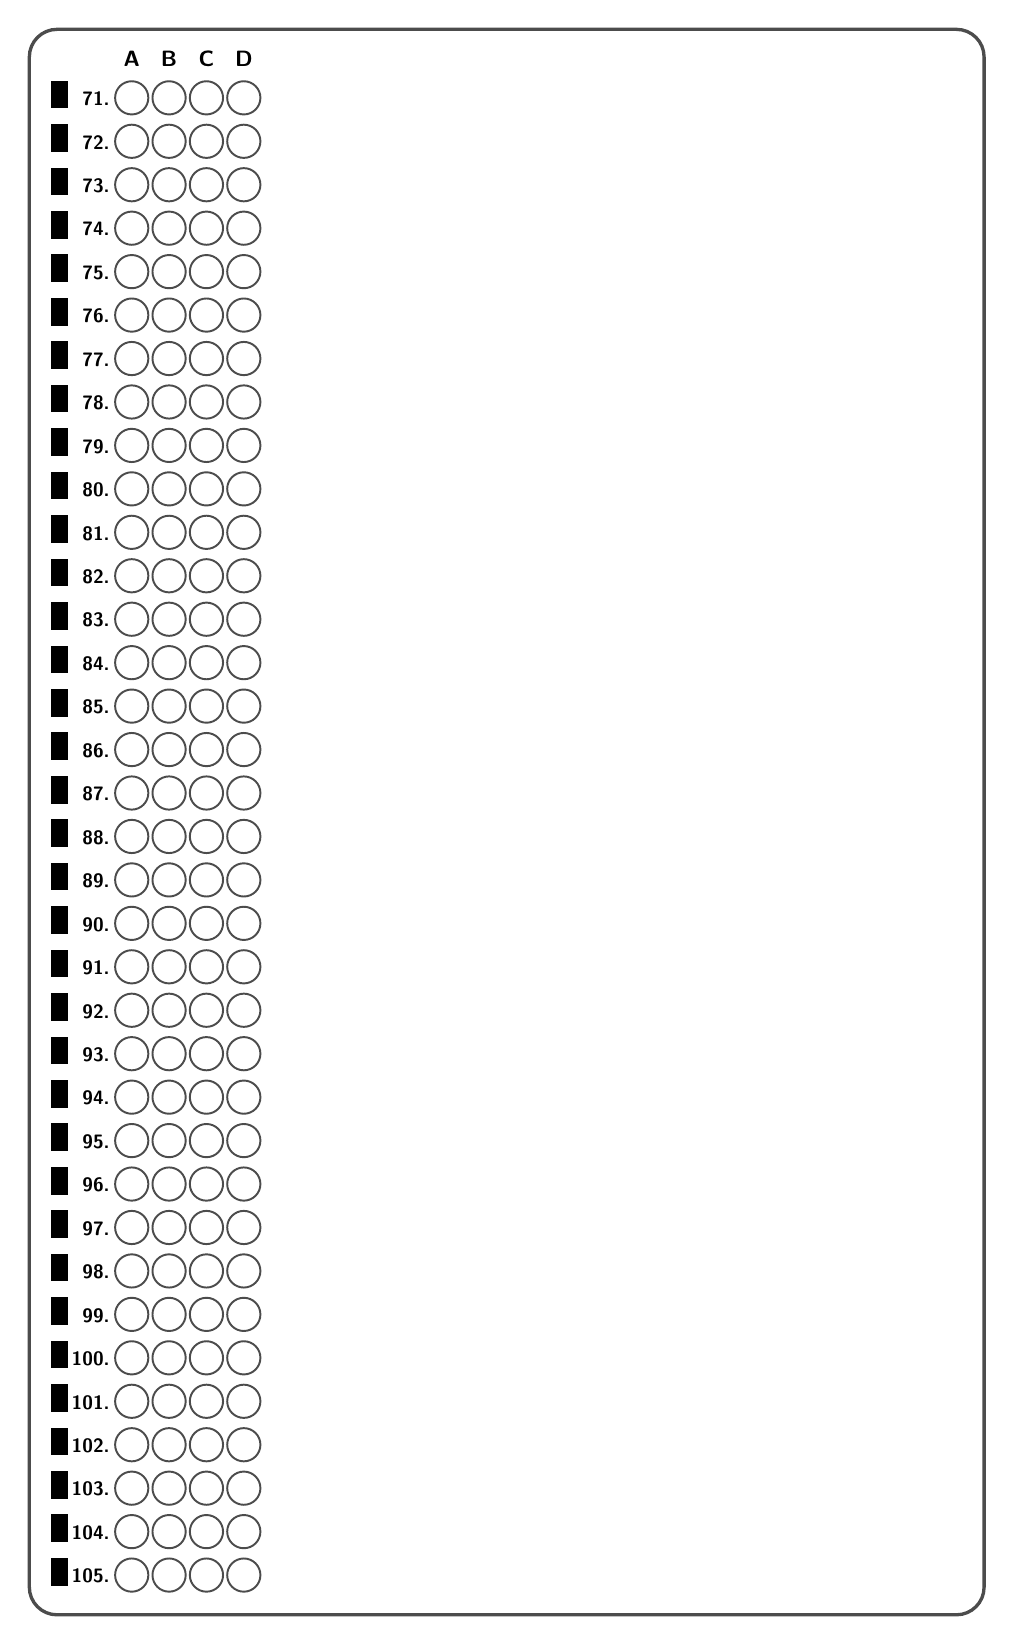
\begin{tikzpicture}
    \node[cuadrocolumna] {
        \HDR
        \foreach \n in {71,...,105}{\Q{\n}}
    };
  \end{tikzpicture}
\end{minipage}%
\hfill
% Columna 4 (MÁS ANCHA para A-H)
\begin{minipage}[t]{0.28\textwidth}
  \vspace{0pt}
  \noindent
  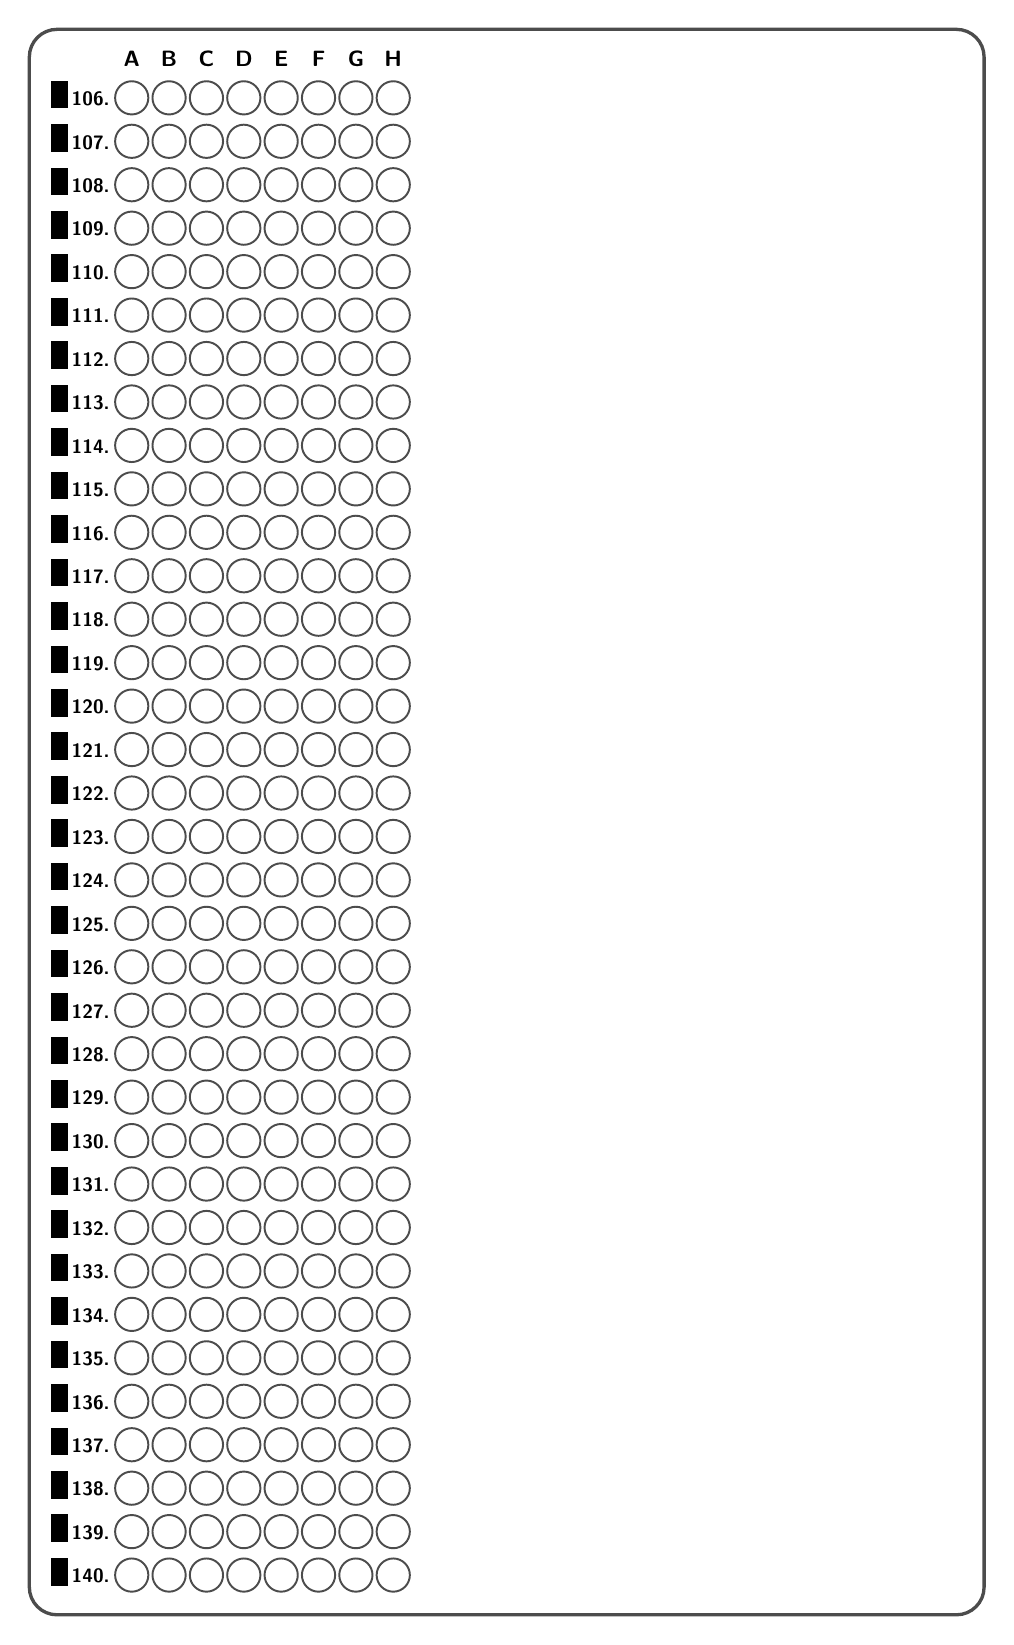
\begin{tikzpicture}
    \node[cuadrocolumna] {
        \HDRH
        \foreach \n in {106,...,140}{\QH{\n}}
    };
  \end{tikzpicture}
\end{minipage}

\end{document}
